% -*- latex -*-
% FILE: "/home/evmik/jobs/wm/2012_spring_Analog_Electronics_252/final_exam/questions/filters_multi_choice.tex"
% LAST MODIFICATION: "Mon, 30 Apr 2012 23:14:28 -0400 (evmik)"
% (C) 2011 by Eugeniy Mikhailov, <evgmik@gmail.com>
% $Id:$

\question{}
	For circuits shown below specify if it a low-pass, high-pass, band-pass
	or band-reject filter. {\bf Hint:} It may be useful to think about
	transfer function at high and low frequencies.
	\begin{parts}
		\part[2]
		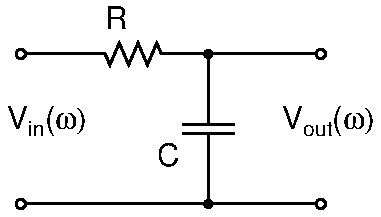
\includegraphics[height=0.7in]{./schematics/rc_low_pass}

		\part[2]
		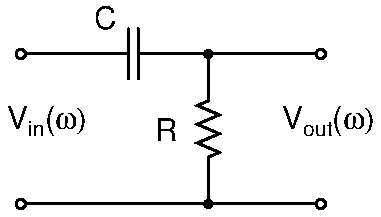
\includegraphics[height=0.7in]{./schematics/rc_high_pass}

		\part[2]
		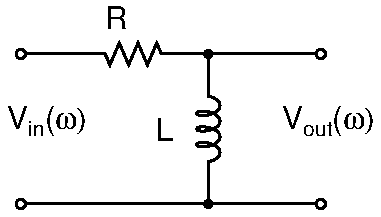
\includegraphics[height=0.7in]{./schematics/rl_high_pass}

		\part[2]
		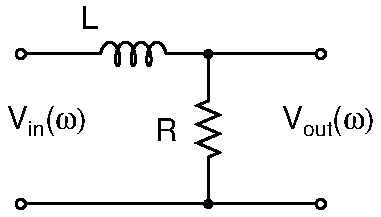
\includegraphics[height=0.7in]{./schematics/rl_low_pass}

		\part[2]
		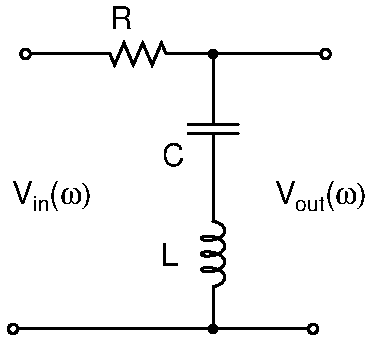
\includegraphics[height=0.7in]{./schematics/rlcnotch}

		\part[2]
		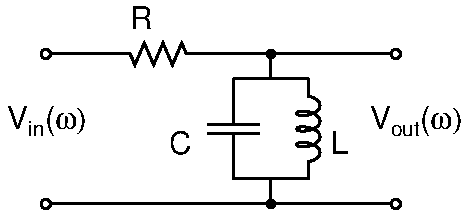
\includegraphics[height=0.7in]{./schematics/rlc_band_pass}

		\part[2]
		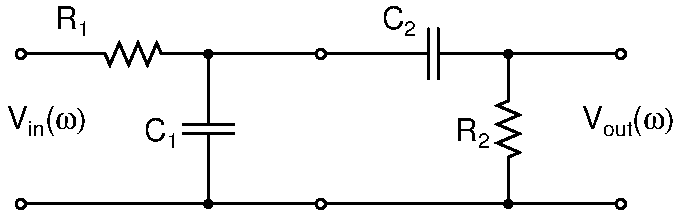
\includegraphics[height=0.7in]{./schematics/band_pass_filter}

		\part[2]
		Sketch the transfer function of the last filter (g)  in log-log
		scale.
		\vskip 1in 

		\part
		Under what conditions the last filter (g) has a transfer
		function close to unity at least in some frequency region?

		\begin{subparts}
			\subpart[2]
				Express one condition in terms of $3_{dB}$ points of the
				low-pass and high-pass filters constituting combined
				filter (g). 
			\vskip 0.5in
			\subpart[2]
				What must be true about $R_1$ and $R_2$?
		\end{subparts}


	\end{parts}
	\pagebreak

